In general, representation types could not be distinguished, meaning model variants of the same specification regarding $\beta$ parameter and algorithm type but with differing representation types were of the same likelihood.
Therefore, representation types will be ignored in the following section, and model likelihoods are capped at $50\%$, because there will always be a tie with the model variant with the other representation type.

\subsection{Experiment 1}
\begin{figure}
	\centering
	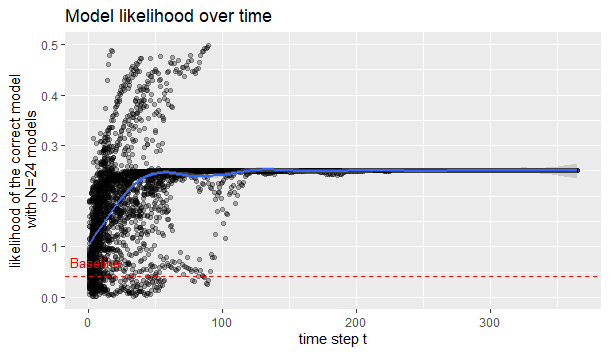
\includegraphics[width=0.95\linewidth]{../../statistics/R_noobst_t_likelihoodall}
	\caption{Likelihood of the true model over the time steps of the trajectories for Experiment 1 with no obstacles and randomized start and goal positions. The p values are drawn in black, whereas the blue line shows the generalized additive model.}
	\label{fig:rnoobsttlikelihoodall}
\end{figure}

Over all 100 trials, the mean length of the trajectories was 62.2 steps (median=13, SD=112.93), with a minimum of 1 step and a maximum of 365 steps.
For models with greedy algorithm type, the mean number of steps was 72.61, whereas for optimal algorithm type, the mean number was 49.98.

Evolution of likelihood for the true, generating model (i.e. the ground truth), over time can be seen in Figure \ref{fig:rnoobsttlikelihoodall}. At the last step of each trajectory, mean likelihood of the true model was .178 (median=.158, SD=.124).

\begin{figure}
	\centering
	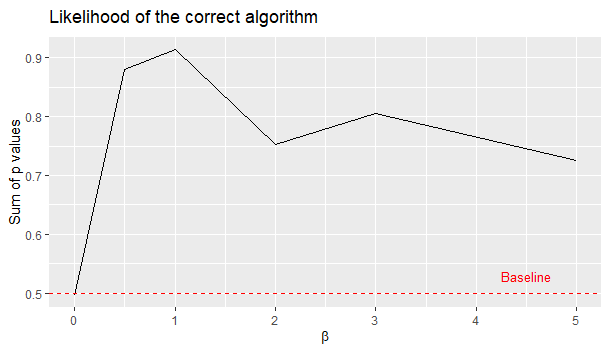
\includegraphics[width=0.95\linewidth]{../../statistics/R_noobst_beta_likelihoodalgo}
	\caption{Likelihood of the correct algorithm in Experiment 1 for all levels of $\beta$, calculated by summing up the p values of all models with the same algorithm as the true model.}
	\label{fig:rnoobstbetalikelihoodalgo}
\end{figure}

The true model is in most cases among the models with the highest likelihood, on average, around 87\% of model variants were worse than the true model (SD= .19).
On average, in 48\% of trials, the true model is among the models with the highest likelihood.
In these cases, all other models with the same likelihood share the same $\beta$ (determinism) factor, but employ the other representation and algorithm types.


Algorithm type could be distinguished, with a certainty of at least $95\%$, in $45\%$ of trials.
A distribution over the different levels for $\beta$ and the respective likelihood of the correct algorithm can be found in Figure \ref{fig:rnoobstbetalikelihoodalgo}.

\begin{figure}
	\centering
	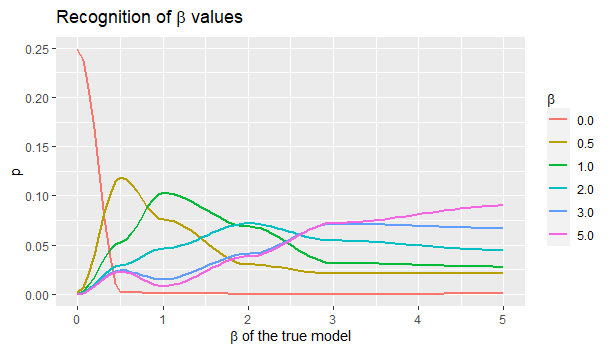
\includegraphics[width=0.95\linewidth]{../../statistics/R_noobst_beta_beta}
	\caption{Summarized p values of all model variants with the specific levels of $\beta$ values for Experiment 1. X axis shows the $\beta$ levels of the true model, colored lines show the local polynomial regression fit of the respective summarized p values of the model variants with specific $\beta$ values.}
	\label{fig:rnoobstbetabeta}
\end{figure}

Likelihoods of the different $\beta$ values relative to the $\beta$ value of the true model can be seen in Figure \ref{fig:rnoobstbetabeta}.



\subsection{Experiment 2}
\subsubsection*{a) Convex Obstacles}

Mean length of the trajectories was 316.6 steps (median=130.5, SD=455.07), with a minimum of 24 steps and a maximum of 2547 steps.
For models with greedy algorithm type, the mean number of steps was 571.4, whereas for optimal algorithm type, the mean number was 81.35.

Evolution of likelihood for the true, generating model, over time can be seen in Figure \ref{fig:rconvextlikelihoodall}. At the last step of each trajectory, mean likelihood of the true model was .365 (median=.434, SD=.145).

The true model is in most cases among the models with the highest likelihood, on average, around 98.7\% of model variants were worse than the true model (SD= .041).
On average, in 89\% of trials, the true model is among the models with the highest likelihood.
In these cases, all other models with the same likelihood share the same $\beta$ (determinism) factor, but employ the other representation type as discussed before.


Algorithm type could be distinguished, with a certainty of at least $95\%$, in $87\%$ of trials.
A distribution over the different levels for $\beta$ and the respective likelihood of the correct algorithm can be found in Figure \ref{fig:rconvexbetaalgosum}.


\begin{figure}
	\centering
	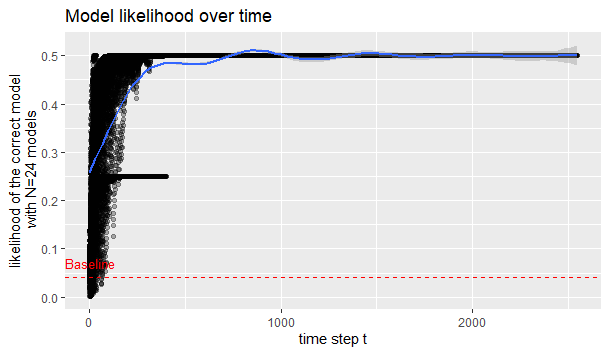
\includegraphics[width=0.95\linewidth]{../../statistics/R_convex_t_likelihoodall_points}
	\caption{Likelihood of the true model over the time steps of the trajectories for Experiment 2a with convex obstacles. The p values are drawn in black, whereas the blue line shows the generalized additive model.}
	\label{fig:rconvextlikelihoodall}
\end{figure}

\begin{figure}
	\centering
	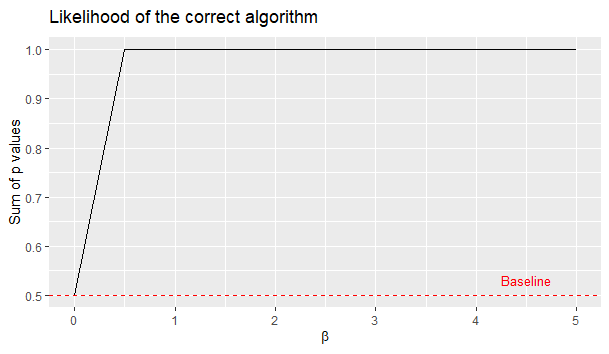
\includegraphics[width=0.95\linewidth]{../../statistics/R_convex_beta_algosum}
	\caption{Likelihood of the correct algorithm in Experiment 2a for all levels of $\beta$, calculated by summing up the p values of all models with the same algorithm as the true model.}
	\label{fig:rconvexbetaalgosum}
\end{figure}

\begin{figure}
	\centering
	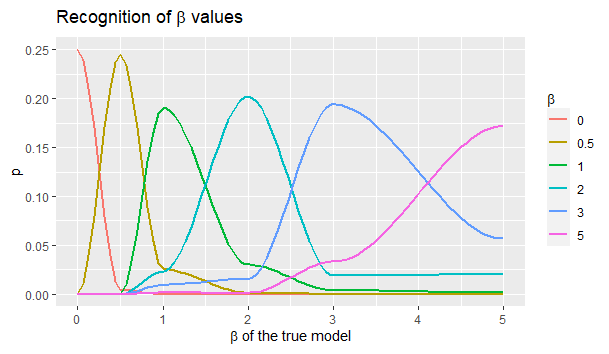
\includegraphics[width=0.95\linewidth]{../../statistics/R_beta}
	\caption{Summarized p values of all model variants with the specific levels of $\beta$ values for Experiment 2a. X axis shows the $\beta$ levels of the true model, colored lines show the local polynomial regression fit of the respective summarized p values of the model variants with specific $\beta$ values.}
	\label{fig:rbetaconvex}
\end{figure}

Likelihoods of the different $\beta$ values relative to the $\beta$ value of the true model can be seen in Figure \ref{fig:rbetaconvex}.

\subsubsection*{b) Concave Obstacles}

During the trials, between 24 and 2460 time steps were taken, with a mean of 499.5 (median=396, SD=536.26).
For models with greedy algorithm type, the mean number of steps was 531, whereas for optimal algorithm type, the mean number was 70.92.

Evolution of likelihood for the true, generating model, over time can be seen in Figure \ref{fig:rtlikelihoodall}. At the last step of each trajectory, mean likelihood of the true model was .388 (median=.5, SD=.144).

The true model is in most cases among the models with the highest likelihood, on average, around 98.6\% of model variants were worse than the true model (SD= .034).
On average, in 84\% of trials, the true model is among the models with the highest likelihood.
In these cases, all other models with the same likelihood share the same $\beta$ (determinism) factor, but employ the other representation type as discussed before.


Algorithm type could be distinguished, with a certainty of at least $95\%$, in $86\%$ of trials.
A distribution over the different levels for $\beta$ and the respective likelihood of the correct algorithm can be found in Figure \ref{fig:rbetaalgosum}.


\begin{figure}
	\centering
	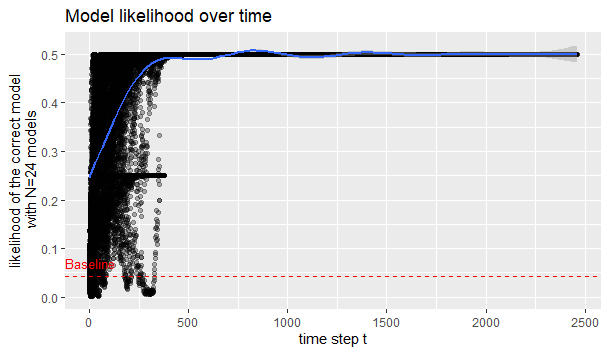
\includegraphics[width=0.95\linewidth]{../../statistics/R_concave_t_likelihoodall_points}
	\caption{Likelihood of the true model over the time steps of the trajectories for Experiment 2b with concave obstacles. The p values are drawn in black, whereas the blue line shows the generalized additive model.}
	\label{fig:rtlikelihoodall}
\end{figure}


\begin{figure}
	\centering
	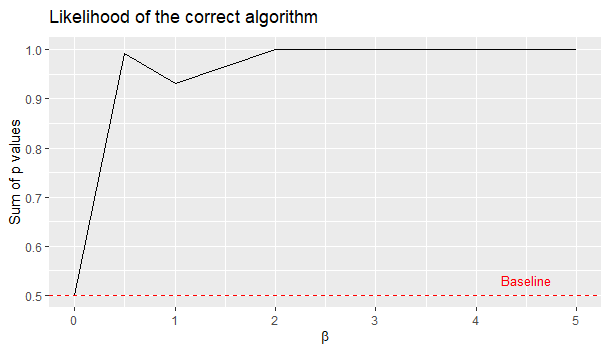
\includegraphics[width=0.95\linewidth]{../../statistics/R_concave_beta_algosum}
	\caption{Likelihood of the correct algorithm in Experiment 2b for all levels of $\beta$, calculated by summing up the p values of all models with the same algorithm as the true model.}
	\label{fig:rbetaalgosum}
\end{figure}

\begin{figure}
	\centering
	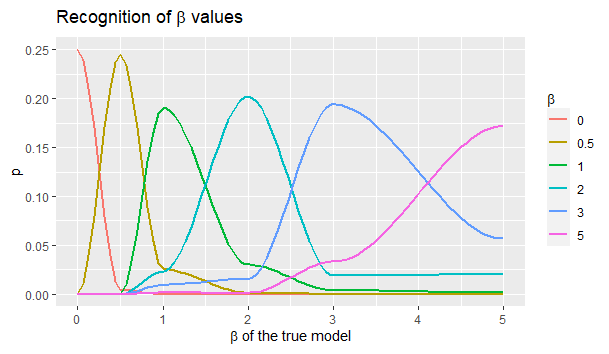
\includegraphics[width=0.95\linewidth]{../../statistics/R_beta}
	\caption{Summarized p values of all model variants with the specific levels of $\beta$ values for Experiment 2b. X axis shows the $\beta$ levels of the true model, colored lines show the local polynomial regression fit of the respective summarized p values of the model variants with specific $\beta$ values.}
	\label{fig:rbeta}
\end{figure}

Likelihoods of the different $\beta$ values relative to the $\beta$ value of the true model can be seen in Figure \ref{fig:rbeta}.
